\section{A Novel Thread Model --- \myth}
\label{sec:design}
%这一部分,首先,我们将详细分析Phoenix较差scalability的根本原因,然后针对Phoenix scalability存在的challenge,我们提出可行的解决方案,即构造一种具有较好scalability的thread model。然后详细解释这种新的线程模型的详细设计方案,最后具体的实验部分在section 6
In this section, we present a new thread model (\myth), which can support \myds to achieve good scalability.
And then, the detail API of \myth will be given.
we focus on the design and implementation of an unboundary channel in \myth.

%we first investigate the main factor of Phoenix's limited scalability,

%\subsection{Analyze Scalability of Phoenix}
%%描述Phoenix 的 pool scalability
%Phoenix utilizes shared-memory multiple threads to implement parallelism, and programs written in Phoenix will start as many threads as the system's cores.
%Ideally, adding more threads and cores to the runtime would bring about a linear decrease in execution time.
%%However, the parallel scalability of Phoenix is not ideal.
%However, Phoenix can not scale as well as expected.
%As indicated in Figure \ref{fig:phoenix:speedup}, when the system exceeds its scalability limitation, adding more cores might scale negatively.
%That means the time of completing a workload will increase if there are more cores in the system. 
%% In general, the parallel scalability of Phoenix is poor.
%
%%使用perf来收集热点函数的执行时间,实验结果显示,在32核情况下,(这里可以给出一个图,16和32核下的热点函数分别是什么,占用多少的百分比分别又是多少?)
%%为了深入探究较差scalability的根本原因,
%%我们利用Linux perf工具来收集程序的热点函数信息(主要看热点函数占用总运行时间的百分比),
%%通过热点函数的分析,查看高核情况下,占用时间最多的运行函数,
%%如表\ref{}显示,在16和32核情况下,各个应用程序中占用时间最多的函数。
%%从表中可以看出,对一hist, lr, wc, sw,在32核情况下ticket\_spin\_lock的开销非常大,
%%针对ticket\_spin\_lock,我们测试各应用程序的占用情况,如图\ref{}所示,
%%从图中可以看出,
%%随着核数的增多,各应用程序中的ticket\_spin\_lock的占用的开销越来越大,
%%特别地,在16核和32核情况下,
%%histgram中ticket\_spin\_lock占用的开销最大,分别为71.25\%和40.15\%.
%%这表明,16核以上,hist, lr, wc, sm的运行时间主要用于锁的竞争和等待,
%%而没有做实际的计算。
%%并且随着核数的增多,这种竞争越激烈,导致Phoenix的scalability较差。
%%事实上,从前面对Phoenix的分析我们知道,
%%Phoenix中采取了划分和barrier两种策略,以避免多个map和reduce对同一个matrix竞争,
%%然而实验的结果却显示在8核以上,依然有很激烈的竞争。
%%函数的调用图显示,ticket\_spin\_lock几乎全部是由pagefault引起的。
%In order to analyze the limited scalability behavior, Linux perf is exploited to collect execution time information of hot function. 
%We note that the map function is the hottest function with less cores, while \_\_ticket\_spin\_lock will become the hottest function with more cores.
%\_\_ticket\_spin\_lock is a type of spinlock which is caused by the contention on the shared structure in Linux kernel.
%In order to specially explore the impact of spinlock in Phoenix, we collect the execution time percent of \_\_ticket\_spin\_lock on each benchmark from 1 to 32 cores by Linux perf.
%
%%However, the structure data shared by multiple threads in Linux kernel can cause the lock contention, which will degrade the scalability of Phoenix.
%%To alleviate the overhead of lock, Phoenix has took two strategies to avoid multiple threads contending the share area.
%%Figure \ref{fig:phoenix:spinlock} shows the execution time percent of \_\_ticket\_spin\_lock on each benchmark. 
%As the result shows in Figure\ref{fig:phoenix:spinlock}, the cost of spinlock increases quickly as the cores number cross a specific value (ie. 8).
%%And in 32 cores, the \_\_ticket\_spin\_lock needs largest execution time for hist, lr, wc, sw.
%%Specially, hist with 16 and 32 cores shows that \_\_ticket\_spin\_lock is the function that has largest execution time percents of 40.15\%  and 71.25\%, respectively. 
%Specially, for hist with 16 and 32 cores, \_\_ticket\_spin\_lock is the function that has largest execution time percents of 40.15\%  and 71.25\%, respectively. 
%Experiment results demonstrate that Phoenix suffers from serious lock contention when the cores number exceeds 8. 
%That means most of execution time will be used for waiting but not actual computation.
%Call-graph information shows that \_\_ticket\_spin\_lock is caused by pagefault, which is not scale well on large numbers of cores.
%
%%	Linux kernel won't scale well on multicores system: 
%%	that applications will spend an increasing fraction of their time in the kernel as the number of cores increases.
%		
%
%
%
%\begin{figure}[!h!t]  
%    \centering
%    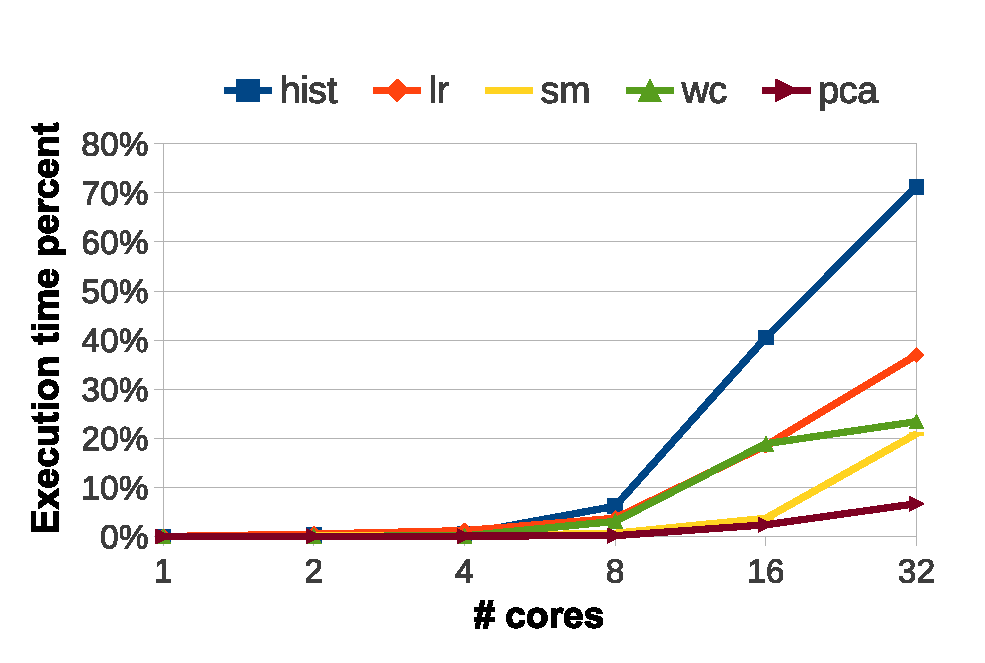
\includegraphics[width=0.45\textwidth]{eps/phoenix_spinlock.eps}
%    \caption{Phoenix ticket\_spin\_lock percent}
%    \label{fig:phoenix:spinlock}
%\end{figure}
%
%
%%Phoenix采取了划分和barrier的方式,以避免多个线程对共享区域的的竞争,为什么还会存在如此高的spinlock呢,
%%\grayt{There is a sense in the community that traditional kernel
%%designs won’t scale well on multicore processors: that
%%applications will spend an increasing fraction of their time
%%in the kernel as the number of cores increases.
%%To understand the Linux scalability
%%behavior, we analyze the related implementation of Linux
%%kernel and exploit performance tools to identify scalability
%%bottlenecks.
%%}
%%and source code analysis
%
%%One reason that widely used operating systems 
%%use a lock on the address space is 
%%that they use complex index data structures to guarantee O(log n)
%%lookup time when a process has many mapped memory
%%regions. Linux uses a red-black tree for the regions\cite{linux}. 
%%Because the data structures require rebalancing 
%%when a memory region is inserted, 
%%they protect the entire data structure with a single lock.
%%The lock is local to a process address space.
%%when the process is using multiple threads 
%%then these threads will be able to access
%%the address space in parallel, 
%%which can cause contention on the lock.
%%%随着核数的增多,这种问题会更加突出,最好导致较差的scalability
%%\bluet{As the increasing of cores number, 
%%	the scalability will be bad.
%%}
%
%
%The mmap() system call is utilized to read in input data. 
%Once the user passes the pointer of the mmap() region to runtime as an argument, multiple map threads will concurrently cause pagefault in the input data when they invoke map functions.
%All of these pagefaults need to access the unique mmap\_sem semaphore, which is local to a process address space. 
%As a result, multiple threads concurrently pagefaults will casue contention to the single semaphore.
%%All these pagefaults will contend the unique mmap\_sem semaphore
%%which is used for protecting the address space shared by multiple threads.
%One reason why Linux uses this single semaphore on the address space is 
%that it needs a red-black tree to guarantee $O$(log$n$)
%lookup time when a process has many mmap memory regions \cite{linux}. 
%%Since the red-black tree requires re-balance when a new memory region is inserted, 
%%Linux protect the entire data structure with a single semaphore.
%%when the process is using multiple threads, 
%%then these threads will be able to access the address space in parallel, 
%%Since the semaphore is local to a process address space, process's multiple threads concurrently access will cause contention on the unique semaphore.
%The semaphore is a sleep lock and may run into convoying problems,
%where waiting threads may get stuck at the end of the wait queue for a long time \cite{Andi2009lmulticore}.
%The contention is intense when there are large amounts of threads,
%which will lead to the parallel scalability degradation on the benchmarks.
%%Therefore, when performing many threads,  the spinlock contention will degrade the parallel scalability performance of the benchmark.
%
%%Data structure private locks can be a problem 
%%if the data structure is shared by multiple threads. 
%%A standard example here are the mm\_sem read-write semaphore 
%%that protects the list of mappings in a process and 
%%the pagetable\_lock that protects the pagetable state of a process. 
%%These locks are local to a process’ address space. 
%%\bluet{In Phoenix, there is one master process,
%%and map worker or reduce worker are threads belong to the master process}. 
%%However when the process is using multiple threads 
%%then these threads will be able to access the address space in parallel,
%%which can cause contention on these locks.
%%Call-graph information
%%and source code analysis show that the two functions are
%%called when adding a virtual memory address range into the
%%process address space or deleting a virtual memory address range. 
%
%
%
%
%%Unfortunately these programs are often written to start as many threads as the system has CPUs, 
%%but when the system is larger than their scalability limit adding more threads might actually scale negatively.
%%The first measure is to limit them to the maximum number of threads that they can successfully scale to.
%%This of course leaves some of the CPUs idle. 
%
%
%
%
%%The difference between processes and threads under Linux 2.4 is that threads share more parts of their state (address space, file handles etc) than processes, 

\subsection{Scalable thread library}
%这一部分,我们不提生产消费模型,
%为什么要进行地址空间隔离,通过新的线程模型,我们实现了地址空间隔离,隔离之后有什么好处?相比Phoenix,我们这种新的模型会不会带来开销。

Our goal is to enable the page faults to be scalable for many cores.
There are some ways to achieve this target. 
For example, Corey\cite{boyd2008corey} is a scalable operating system for multicore;
Clements et.al. proposed a scalable address spaces by using RCU balanced trees \cite{Clements2012Scalable};
Andi et.al think process has a better scalability than thread since the process needs not to share the address space with the other processes\cite{Andi2009lmulticore}.
%applications use processes instead of threads can avoid a single shared address space
However, modifying operation system is impracticable and employing the process rather than the thread will make sharing become complicated. 
In order to provide a practicable and simple solution, a key problem to be solved is that how to enable threads to eliminate contention on the per-process read/write semaphore when multiple threads concurrently run page faults and \codet{mmap} operations.



%This requires addressing a basic problem, how allow pagefaults to eliminate on the per-process read/write semaphore, when multiple threads run concurrently.
%At the same time, we aim at providing an easy-to-use programming abstraction to support scalable MapReduce.
%The proposed \myth can support scalable MapReduce (\myds).


%we persents a new concurrent address space design 
%that eliminates the above sources of contention by applying a new program model and by introducing channel, a way to share data between threads.
%We aim at providing an easy-to-use programming abstraction to support scalable MapReduce.
%With this target, we propose a new thread programming model \myth(Scalable thread).
%We propose a new thread programming model to support efficient pipeline parallelism.
%To address this issue and achieve our goal, we propose a new thread programming model \myth(Scalable thread), which is written in C.
To address the problem and achieve our goal, we propose a novel thread programming model \myth (Scalable thread) with better scalability, supporting scalable MapReduce (\myds) compatibly.
%will be presented in this subsection.
There are two key points in the design of \myth.
Firstly, we confine the threads in \myth to run in separate memory spaces to avoid the contention.
It means that threads in \myth have their local \codet{mmap\_sem} and eliminate the contention of the single semaphore with others thread.
Secondly, when using the separate memory spaces, communication will be challenging since the threads in \myth can not directly communicate with the other threads like thread based on share space.
So, we give a \chan for the threads to communicate with the others in \myth. 
%Threads in Pthreads share the address space of the process that created it, 
%while threads in \myth have their own address space,
%meaning each thread has a mm\_struct.
%Therefore, thread no need contend with others thread for lock.

%While \myth must use interprocess communication to communicate with the other threads.



\label{sec:pm:thread}
\begin{figure}[htpb]
\input chanapi.tex
\caption{Main functions of \myth thread API}
\label{fig:api:thread}
\end{figure}

%mapreduce中是如何使用这个简易的模型进行编程和实现的,这个模型潜在的开销是什么
Figure \ref{fig:api:thread} lists the main functions of managing threads and channels in \myth.
In the case of \myds, at initial stage, the master thread invokes \codet{thread\_alloc} to allocate map threads and reduce threads, and then creates the \chan  between each pair of map and reduce threads by invoking \codet{chan\_alloc}.
%To set up the shared-channel, the master invokes \codet{chan\_setprod} and \codet{chan\_setcons} to set the map and reduce threads as producers and consumers, respectively. 
After that, the master invokes \codet{chan\_setprod} and \codet{chan\_setcons} to set the map and reduce threads as producers and consumers for the shared-channel, respectively.
The producer sends messages to the \chan, and the consumer receives the messages from it,
which is a typical producer-consumer model (we will detail how it will be used in Section 4). 
Finally, the master starts all threads to work by invoking \codet{thread\_start}.

Although \myth can decrease the overhead of contention,
it also takes extra overhead in comparison to Phoneix. The experiments demonstrate that the extra overhead 
is concentrate in the initial stage (we will analyze this overhead in Section 5.3). 


\subsection{Unboundary Channel}
%channel的底层实现,以及它无限制的映射机制,想说明的问题是:不需要等待,且没有过多的malloc和free操作带来的开销。
%Once the producer and consumer thread have been created and channel relationships are set,
In our design, the \chan is a virtual memory area, called \code{CHAN} in the producer and consumer address space.
When the producer invokes \code{chan\_send} to send data, the sent data will be copyed to the \code{CHAN} area.
And then the consumer reads the data from the \code{CHAN} area  by invoking \code{chan\_recv}.
There is a pagetable (\code{ptab}) used to store the mapping between \code{CHAN} memory area and physical address, with each mapping as a corresponding page table entry.

%Once the channel relationships are set up, 
%the producer can invoke \codet{chan\_send} to send key-value to corresponded channel,
%and the reduce workers can receive from the channel by \codet{chan\_recv}.
%In order to avoid the producer waiting when the channel buffer is full,
%we design an unbounded size of communication buffer for channel.
%That means a sender can send any number of messages without blocking or waiting.
%As a result, system can achieve high throughput.
%Unboundedness goal is the key to achieve high throughput.
%这个特性的好处


%无边界的channel的实现,依赖于底层的extend机制,
%它允许将channel buffer区域重新映射到一块新的物理地址,
%并且不影响consumer对旧的物理的读取。
%channel buffer对应producer和consumer地址空间中一块区域,
%我们称之为\codet{CHAN}区域,有一个pagetable(\codet{ptab})用于管理该区域的物理地址映射。
\begin{figure}[!h!t]  
	\centering
	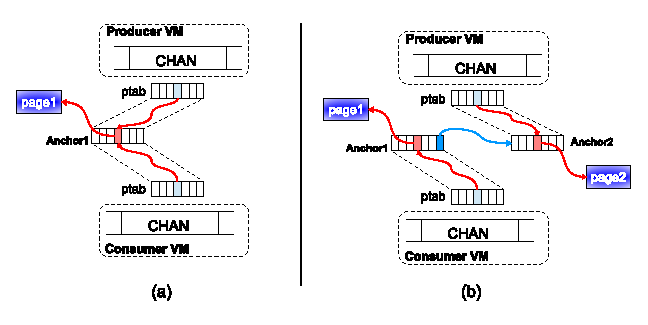
\includegraphics[width=0.45\textwidth]{eps/chan_extend.eps}
	\caption{channel extend machanism}
	\label{fig:spmckern:extend}
\end{figure}

%extension
Initially, as shown in Figure \ref{fig:spmckern:extend}(a), the runtime will not allocate the actual page frames for \code{CHAN} area but map it to a special page frame--- anchor page table (\code{Anchor1}) which is shared by the producer and consumer.
Meanwhile, each entry in the \code{ptab} of both the producer and consumer will point to the same entry in \code{Anchor1}. 

%That is each entry(pte) in \code{ptab} points to the address of Anchor1(Anchor1 in Figure\ref{fig:spmckern:extend}(a)).
When the producer sends data, the runtime attempts to write the sent data into the \code{CHAN} area, which will trigger a pagefault. 
%writing the data to CHAN, a pagefault will take place.
Then the pagefault handler will allocate a page frame (\code{page1}) for the producer, and the corresponding \code{pte} in \code{Anchor1} will be updated to point to the allocated page (\code{page1}). 
%After that, the runtime can copy the sended data to the page(\code{page1}).
%Then producer can locate the page by \code{pte} and the data need to send will copy to this \code{page1} lastly.
After that, the consumer can locate the page frame \code{page1}  and then read data from \code{page1} by by the anchor page (\code{Anchor1}).


In general producer-consumer model, if the channel buffer is full, the producer needs to wait until the consumer removes the data from it, which limits the performance and throughput of the system.
To avoid the producer waiting, we design a channel buffer with unbounded size  by exploiting an \codet{extend} mechanism\cite{zhang13lazy}.
This mechanism allows the producer uninterruptedly sending data with no need for waiting.
This \codet{extend} mechanism (Figure  \ref{fig:spmckern:extend}(b)) will remap the channel buffer (i.e., \code{CHAN} area) to another anchor and allocate some new page frames for the producer. 
At the same time, the consumer will not be disturbed and it can continuously read the data from the original page frames.
%Then the runtime will allocate the page frame(\codet{page2}) for the producer, which will be recorded in corresponding \code{Anchor2}'s PTE.
To record and trace the original  and  new page frames, an extension pte is introduced (\code{extension\_pte}).
When the consumer receives all data from the original page frames, it will locate the new page frames by the \code{extension\_pte}.
The original page frames will decrease their reference counts and are automatically freed  when the counts reach zero.


%and consumer can read the old page frames at the same time.
%In order to reach a unbounded buffer,

%but just remap \code{CHAN} to another anchor \code{Anchor2},
%so that the producer can write the page afterwards.
%To record and trace generations of page frames among old page frames 
%and new page frames, a extension PTE is introduced.
%That mean,
%it can call extend primitive to remap channel buffer to new page frames,
%without changing the old page that consumers may still require. 
%Consumer can use the extension \code{pte} to locate the new
%After a consumer receive the old page from the channel, 
%it can call extend to find the new page frames sended by the
%producer.
%The older page frames decrease their reference counts and
%are freed automatically when the counts reach zero.


%a special anchor extension page is introduced and shared between producer thread and consumers consumer.
%Initially a sequence of pages in channel buffer 
%are mapped to a \codet{anchor} page table (Anchor in Figure
%\ref{fig:spmckern:extend}), 
%in which each page has a corresponding page table entry (PTE).
%Upon a producer page fault, the fault handler will allocate a real page frame and update the faulting page with a
%writable producer mapping so that the producer can write the
%page afterwards.
%When a thread want to send without waiting, 
%it can call extend primitive to remap channel buffer to new page frames,
%without changing the old page 
%that consumers may still require. 


In conclusion, we design a scalable thread model (\myth) and provide an unbounded \chan for threads to communicate. This unbounded \chan is a prominent feature of \myth, which is the main difference between our \myth and the previous works. 
We will detail how to sufficiently exploit this feature to implement the scalable MapReduce (\myds)  in Section 4.
%That means a sender can send any number of messages without blocking or waiting.
%As a result, system can achieve high throughput.
%Unboundedness goal is the key to achieve high throughput.








